\documentclass{article}
\pagestyle{plain}
\usepackage{amsmath}
\usepackage{amssymb}
\usepackage{graphicx}
\usepackage[retainorgcmds]{IEEEtrantools}
\begin{document}
\title{Assignment 5 - Differential Equations }
\date{\today}
\author{Mohan S Nayaka}
\renewcommand{\arraystretch}{1.5}
\maketitle

1. \textbf{An example of a second order differential equation describing a natural phenomenon.}

An \textbf{RLC circuit} (or \textbf{LCR circuit}) is an electrical circuit consisting of a resistor, an inductor, and a capacitor, connected in series or in parallel. The RLC part of the name is due to those letters being the usual electrical symbols for resistance, inductance and capacitance respectively. The main difference between this and an LC circuit that the presence of the resistor makes is that any oscillation induced in the circuit will die away over time if it is not kept going by a source. This effect of the resistor is called damping.

\begin{figure}[ht]
\centering
\includegraphics[scale=0.25]{rlcpic}
\caption{A series RLC circuit}
\end{figure}
In this circuit, the three components are all in series with the voltage source. The governing differential equation can be found by substituting into Kirchhoff's voltage law (KVL) the constitutive equation for each of the three elements.
\\From KVL,\\
\[v_R + v_L + v_C = v(t)\]
where $v_R, v_L, v_C$  are the voltages across R, L and C respectively and $v(t)$ is the time varying voltage from the source. Substituting in the constitutive equations,\\
\[Ri(t) + L\frac{di}{dt} + \frac{1}{C}\int_{-\infty}^{\tau=t}i(\tau)d\tau = v(t)\]
For the case where the source is an unchanging voltage, differentiating and dividing by L leads to the second order differential equation:
\[\frac{d^2i(t)}{dt^2}+\frac{R}{L}\frac{di(t)}{dt} + \frac{1}{LC}i(t) = 0\]
This can usefully be expressed in a more generally applicable form:
\begin{equation}
\frac{d^2i(t)}{dt^2}+2\alpha\frac{di(t)}{dt} + \omega_0^2i(t) = 0 \label{maineq}
\end{equation}
$\alpha$ and $\omega_0$ and  are both in units of angular frequency. $\alpha$ is called the neper frequency, or attenuation, and is a measure of how fast the transient response of the circuit will die away after the stimulus has been removed. Neper occurs in the name because the units can also be considered to be nepers per second, neper being a unit of attenuation. $\omega_0$  is the angular resonance frequency.
For the case of the series RLC circuit these two parameters are given by:\\
\[\alpha = \frac{R}{2L} \text{ and } \omega_0=\frac{1}{\sqrt{LC}}\]
A useful parameter is the \textit{damping factor}, $\zeta$ which is defined as the ratio of these two,\\
\[\zeta=\frac{\alpha}{\omega_0}\]
In the case of the series RLC circuit, the damping factor is given by,\\
\[\zeta=\frac{R}{2}\sqrt{\frac{C}{L}} \]\\
\pagebreak
\begin{center}
\textbf{Transient Response}
\end{center}
The form of the solution of the differential equation \eqref{maineq} for the circuit depends on the value of $\zeta$. There can be three cases:\\
\begin{enumerate}
\item underdamped : $\zeta$ $<$ 0
\item overdamped  : $\zeta$ $>$ 0
\item critically damped :  $\zeta$ = 0
\end{enumerate}
The differential equation \eqref{maineq} has the characteristic equation:\\
\begin{equation*}
s^2 +2\alpha s+\omega_0^2=0
\end{equation*}
The roots of the characteristic equation are:\\
\[s_1=-\alpha+\sqrt{\alpha^2-\omega_0^2}\]
\[s_1=-\alpha-\sqrt{\alpha^2-\omega_0^2}\]
The general solution of the differential equation is an exponential in either root or a linear superposition of both,\\
\[i(t)=A_1e^{s_1t}+A_2e^{s_2t}\]
The coefficients $A_1$ and $A_2$ are determined by the boundary conditions of the specific problem being analysed. That is, they are set by the values of the currents and voltages in the circuit at the onset of the transient and the presumed value they will settle to after infinite time.\\
\\
\textbf{Overdamped Response}
The overdamped response ($\zeta > 0$) is:\\
\[i(t)=A_1e^{-\omega_0(\zeta+\sqrt{\zeta^2-1})t}+A_2e^{-\omega_0(\zeta-\sqrt{\zeta^2 - 1})t}\]
The overdamped response is a decay of the transient current without oscillation.\\
\\
\textbf{Underdamped Response}
The overdamped response ($\zeta < 0$) is:\\
\[i(t)=B_1e^{-\alpha t}cos(\omega_d t) + B_2e^{-\alpha t}sin(\omega_d t)\]
The underdamped response is a decaying oscillation at frequency $\omega_d$.The oscillation decays at a rate determined by the attenuation $\alpha$The exponential in $\alpha$describes the envelope of the oscillation. $B_1$ and $B_2$ are constants determined by the boundary conditions.The frequency $\omega_d$ is given by:\\
\[\omega_d = \sqrt{\omega_0^2 - \alpha_0^2} = \omega_0\left(\sqrt{1-\zeta^2}\right)\]
This is called the damped resonance frequency or the damped natural frequency. It is the frequency the circuit will naturally oscillate at if not driven by an external source. The resonance frequency,$\omega_0$, which is the frequency at which the circuit will resonate when driven by an external oscillation, may often be referred to as the undamped resonance frequency to distinguish it.\\
\\
\textbf{Critical Damped Response}
The overdamped response ($\zeta = 0$) is:\\
\[i(t)=D_1te^{-\alpha t}+D_2e^{-\alpha t}\]
The critically damped response represents the circuit response that decays in the fastest possible time without going into oscillation. This consideration is important in control systems where it is required to reach the desired state as quickly as possible without overshooting. $D_1$ and $D_2$ are  arbitrary constants determined by boundary conditions.
\begin{figure}[hb]
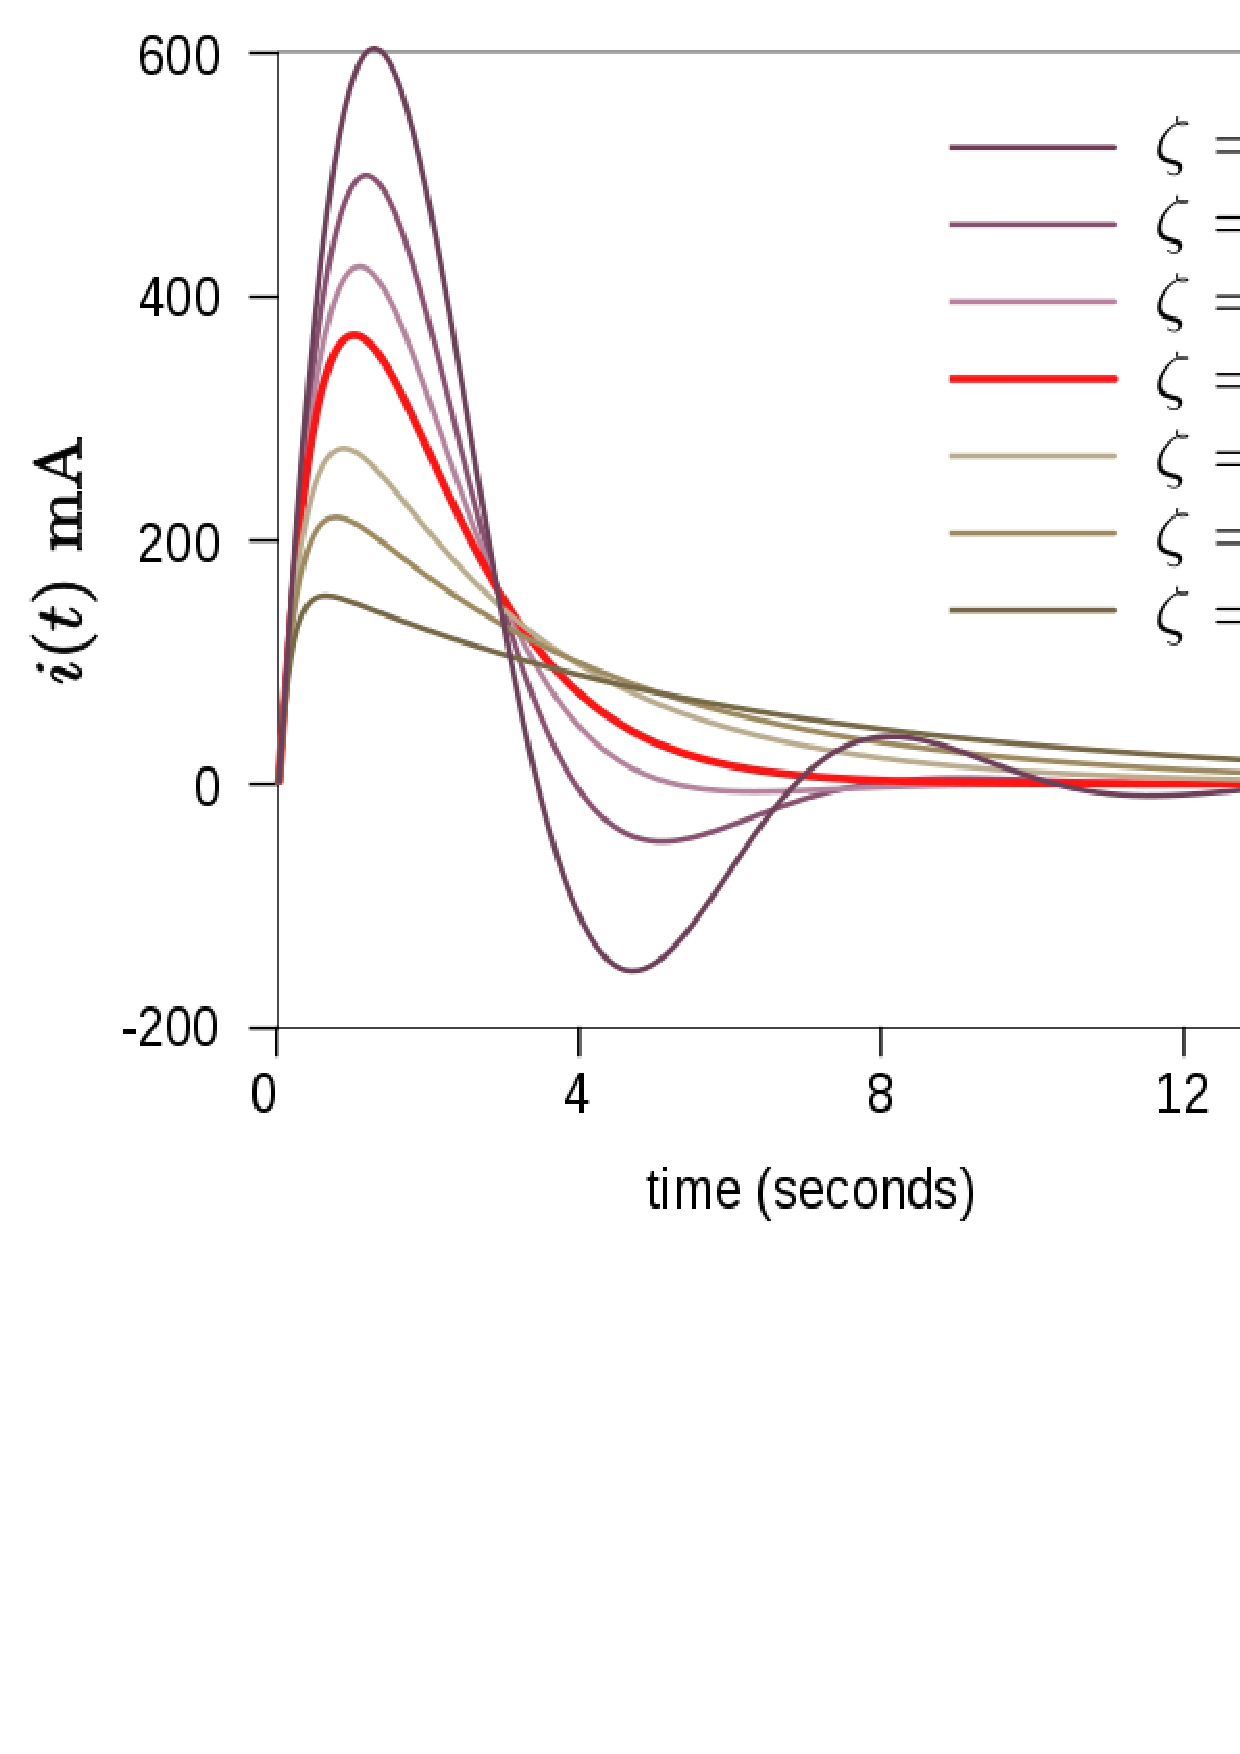
\includegraphics[scale=0.35]{rlcplot}
\caption{Plot showing underdamped, overdamped and critically damped responses}
\end{figure}\\
\\
2. \textbf{Solve the differential equation}:\\
\[y''+2y'+2y=0\]
Given the initial values\\
\[y\left(\frac{\pi}{4}\right)=2 \]\\
\[ y'\left(\frac{\pi}{4}\right)=-2\]

\textbf{Solution}:
The characteristic equation for the given ODE is:\\
\[\lambda^2 + 2\lambda+2 =0\\\]
\begin{align*}
\therefore (\lambda+1)^2  + 1 &= 0\\
\therefore (\lambda+1)^2  &= -1\\
\therefore \lambda+1 &= \pm i\\
\therefore \lambda &= -1 \pm i\\
\end{align*}
Comparing with the solution in the case of complex conjugate roots $\lambda=s+it$,
\[y=e^{sx}(C_1 cos(tx) + C_2 sin(tx))\]
We have,\\
\begin{equation}
y=e^{-x}(C_1 cos(x) + C_2 sin(x)) \label{solmain}
\end{equation}
Applying the initial condition $y(\pi/4)=2$,\\
\[2=e^{-\pi / 4}(C_1 cos (\pi/4)+C_2 sin(\pi/4))\]
Solving, we get\\
\[2=0.4559\left(\frac{C_1}{\sqrt{2}}+\frac{C_2}{\sqrt{2}}\right)\]
\begin{equation}
C_1+C_2=6.204 \label{eqone}
\end{equation}
We differentiate the solution (equation \eqref{solmain}) to apply the second initial value condition,\\
\begin{IEEEeqnarray*}{rCl}
y'&=&e^{-x}(-C_1sin(x)+C_2cos(x))-e^{-x}(C_1cos(x)+C_2sin(x))\\
    &=&e^{-x}(-C_1sin(x)-C_1cos(x)+ C_2cos(x)-C_2sin(x))\\
    &=&e^{-x}(-C_1(cos(x)+sin(x))+C_2(cos(x)-sin(x)))\\
\end{IEEEeqnarray*}
Applying the second initial value condition to the above equation, we get:\\
\begin{IEEEeqnarray*}{rCl}
y'(\pi/4) &=& -2 \\ &=& e^{-\pi/4}(-C_1\left(cos\left(\pi/4\right)+sin\left(\pi/4\right)\right)+C_2(cos\left(\pi/4\right)-sin\left(\pi/4\right)))\\
&=& 0.4559 \left(-C_1\left(\frac{1}{\sqrt2} + \frac{1}{\sqrt2}\right) + C_2\left(\frac{1}{\sqrt2} - \frac{1}{\sqrt2}\right)\right)\\
\end{IEEEeqnarray*}
\[\therefore C_1 = \frac{\sqrt 2}{0.4559}\]
\begin{center}
$\therefore$
\begin{tabular}{|c|}
\hline
$C_1$ = 3.101\\
\hline
\end{tabular}
\end{center}
Substituting this in \eqref{eqone}, we get:\\
\[3.101 + C_2 = 6.204\]
\begin{center}
$\therefore$
\begin{tabular}{|c|}
\hline
$C_2$ = 3.103\\
\hline
\end{tabular}
\end{center}
Hence the solution is:\\
\begin{center}
\begin{tabular}{|c|}
\hline
$y=e^{-x}(3.101 cos(x) + 3.103 sin(x))$\\
\hline
\end{tabular}
\end{center}

\end{document}
